% Options for packages loaded elsewhere
\PassOptionsToPackage{unicode}{hyperref}
\PassOptionsToPackage{hyphens}{url}
%
\documentclass[
]{article}
\usepackage{amsmath,amssymb}
\usepackage{lmodern}
\usepackage{iftex}
\ifPDFTeX
  \usepackage[T1]{fontenc}
  \usepackage[utf8]{inputenc}
  \usepackage{textcomp} % provide euro and other symbols
\else % if luatex or xetex
  \usepackage{unicode-math}
  \defaultfontfeatures{Scale=MatchLowercase}
  \defaultfontfeatures[\rmfamily]{Ligatures=TeX,Scale=1}
\fi
% Use upquote if available, for straight quotes in verbatim environments
\IfFileExists{upquote.sty}{\usepackage{upquote}}{}
\IfFileExists{microtype.sty}{% use microtype if available
  \usepackage[]{microtype}
  \UseMicrotypeSet[protrusion]{basicmath} % disable protrusion for tt fonts
}{}
\makeatletter
\@ifundefined{KOMAClassName}{% if non-KOMA class
  \IfFileExists{parskip.sty}{%
    \usepackage{parskip}
  }{% else
    \setlength{\parindent}{0pt}
    \setlength{\parskip}{6pt plus 2pt minus 1pt}}
}{% if KOMA class
  \KOMAoptions{parskip=half}}
\makeatother
\usepackage{xcolor}
\usepackage[margin=1in]{geometry}
\usepackage{color}
\usepackage{fancyvrb}
\newcommand{\VerbBar}{|}
\newcommand{\VERB}{\Verb[commandchars=\\\{\}]}
\DefineVerbatimEnvironment{Highlighting}{Verbatim}{commandchars=\\\{\}}
% Add ',fontsize=\small' for more characters per line
\usepackage{framed}
\definecolor{shadecolor}{RGB}{248,248,248}
\newenvironment{Shaded}{\begin{snugshade}}{\end{snugshade}}
\newcommand{\AlertTok}[1]{\textcolor[rgb]{0.94,0.16,0.16}{#1}}
\newcommand{\AnnotationTok}[1]{\textcolor[rgb]{0.56,0.35,0.01}{\textbf{\textit{#1}}}}
\newcommand{\AttributeTok}[1]{\textcolor[rgb]{0.77,0.63,0.00}{#1}}
\newcommand{\BaseNTok}[1]{\textcolor[rgb]{0.00,0.00,0.81}{#1}}
\newcommand{\BuiltInTok}[1]{#1}
\newcommand{\CharTok}[1]{\textcolor[rgb]{0.31,0.60,0.02}{#1}}
\newcommand{\CommentTok}[1]{\textcolor[rgb]{0.56,0.35,0.01}{\textit{#1}}}
\newcommand{\CommentVarTok}[1]{\textcolor[rgb]{0.56,0.35,0.01}{\textbf{\textit{#1}}}}
\newcommand{\ConstantTok}[1]{\textcolor[rgb]{0.00,0.00,0.00}{#1}}
\newcommand{\ControlFlowTok}[1]{\textcolor[rgb]{0.13,0.29,0.53}{\textbf{#1}}}
\newcommand{\DataTypeTok}[1]{\textcolor[rgb]{0.13,0.29,0.53}{#1}}
\newcommand{\DecValTok}[1]{\textcolor[rgb]{0.00,0.00,0.81}{#1}}
\newcommand{\DocumentationTok}[1]{\textcolor[rgb]{0.56,0.35,0.01}{\textbf{\textit{#1}}}}
\newcommand{\ErrorTok}[1]{\textcolor[rgb]{0.64,0.00,0.00}{\textbf{#1}}}
\newcommand{\ExtensionTok}[1]{#1}
\newcommand{\FloatTok}[1]{\textcolor[rgb]{0.00,0.00,0.81}{#1}}
\newcommand{\FunctionTok}[1]{\textcolor[rgb]{0.00,0.00,0.00}{#1}}
\newcommand{\ImportTok}[1]{#1}
\newcommand{\InformationTok}[1]{\textcolor[rgb]{0.56,0.35,0.01}{\textbf{\textit{#1}}}}
\newcommand{\KeywordTok}[1]{\textcolor[rgb]{0.13,0.29,0.53}{\textbf{#1}}}
\newcommand{\NormalTok}[1]{#1}
\newcommand{\OperatorTok}[1]{\textcolor[rgb]{0.81,0.36,0.00}{\textbf{#1}}}
\newcommand{\OtherTok}[1]{\textcolor[rgb]{0.56,0.35,0.01}{#1}}
\newcommand{\PreprocessorTok}[1]{\textcolor[rgb]{0.56,0.35,0.01}{\textit{#1}}}
\newcommand{\RegionMarkerTok}[1]{#1}
\newcommand{\SpecialCharTok}[1]{\textcolor[rgb]{0.00,0.00,0.00}{#1}}
\newcommand{\SpecialStringTok}[1]{\textcolor[rgb]{0.31,0.60,0.02}{#1}}
\newcommand{\StringTok}[1]{\textcolor[rgb]{0.31,0.60,0.02}{#1}}
\newcommand{\VariableTok}[1]{\textcolor[rgb]{0.00,0.00,0.00}{#1}}
\newcommand{\VerbatimStringTok}[1]{\textcolor[rgb]{0.31,0.60,0.02}{#1}}
\newcommand{\WarningTok}[1]{\textcolor[rgb]{0.56,0.35,0.01}{\textbf{\textit{#1}}}}
\usepackage{graphicx}
\makeatletter
\def\maxwidth{\ifdim\Gin@nat@width>\linewidth\linewidth\else\Gin@nat@width\fi}
\def\maxheight{\ifdim\Gin@nat@height>\textheight\textheight\else\Gin@nat@height\fi}
\makeatother
% Scale images if necessary, so that they will not overflow the page
% margins by default, and it is still possible to overwrite the defaults
% using explicit options in \includegraphics[width, height, ...]{}
\setkeys{Gin}{width=\maxwidth,height=\maxheight,keepaspectratio}
% Set default figure placement to htbp
\makeatletter
\def\fps@figure{htbp}
\makeatother
\setlength{\emergencystretch}{3em} % prevent overfull lines
\providecommand{\tightlist}{%
  \setlength{\itemsep}{0pt}\setlength{\parskip}{0pt}}
\setcounter{secnumdepth}{-\maxdimen} % remove section numbering
\ifLuaTeX
  \usepackage{selnolig}  % disable illegal ligatures
\fi
\IfFileExists{bookmark.sty}{\usepackage{bookmark}}{\usepackage{hyperref}}
\IfFileExists{xurl.sty}{\usepackage{xurl}}{} % add URL line breaks if available
\urlstyle{same} % disable monospaced font for URLs
\hypersetup{
  pdftitle={Next Generation Sequencing (NGS) ity Analysis with Emoji},
  hidelinks,
  pdfcreator={LaTeX via pandoc}}

\title{Next Generation Sequencing (NGS) ity Analysis with Emoji}
\usepackage{etoolbox}
\makeatletter
\providecommand{\subtitle}[1]{% add subtitle to \maketitle
  \apptocmd{\@title}{\par {\large #1 \par}}{}{}
}
\makeatother
\subtitle{Developed by: Ray Enke, Rachael St.~Jaques1, Max Maza, Caylin
Murray, Sabrina Robertson, Andrew Lonsdale, \& Jason Williams. Modified
by Bárbara Bitarello}
\author{}
\date{\vspace{-2.5em}}

\begin{document}
\maketitle

{
\setcounter{tocdepth}{2}
\tableofcontents
}
\hypertarget{goals}{%
\subsection{Goals}\label{goals}}

\begin{itemize}
\tightlist
\item
  Introduce students to writing basic command line scripts
\item
  Analyze \& assess the quality of FASTQ formatted NGS data
\item
  Trim/filter low quality reads in FASTQ files
\end{itemize}

\textbf{FastQC} is a popular software used to provide an overview of
basic quality metrics for NGS data. In this lesson, you will use an even
more universal form of communication to analyze FASTQ files, THE EMOJI!

\hypertarget{background}{%
\subsection{Background}\label{background}}

\hypertarget{fastq-files}{%
\subsubsection{FASTQ files}\label{fastq-files}}

\begin{itemize}
\item
  The 1st step of any Next Generation Sequencing (NGS) analysis pipeline
  is \textbf{checking the quality of the raw sequencing reads} in each
  FASTQ formatted file. If the sequence quality is poor, then your
  resulting downstream analysis will be inaccurate and misleading.
\item
  The name FASTQ comes from FASTA. FASTA is a very populat format to
  store sequence information (DNA, RNA, proteins).
\end{itemize}

\begin{figure}
\centering
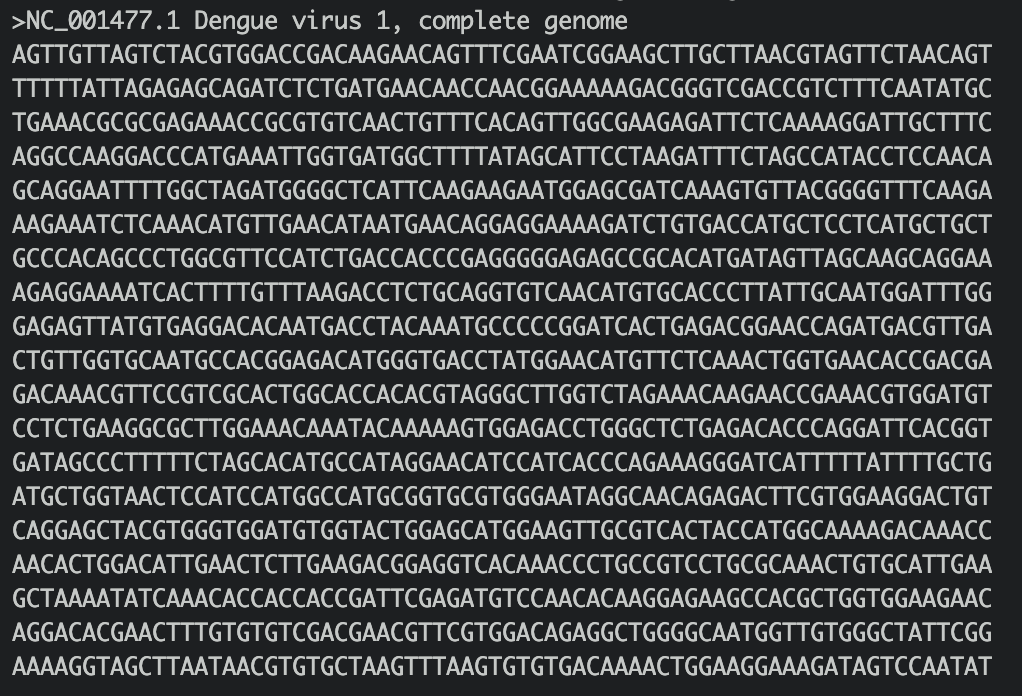
\includegraphics[width=0.7\textwidth,height=\textheight]{images/fastafile.png}
\caption{A part of a FASTA file containing the entire genome of the
dengue virus.}
\end{figure}

\begin{itemize}
\item
  The \texttt{Q} refers to ``quality''.
\item
  Most sequencing platforms will provide raw reads to the user in this
  format.
\end{itemize}

\begin{figure}
\centering
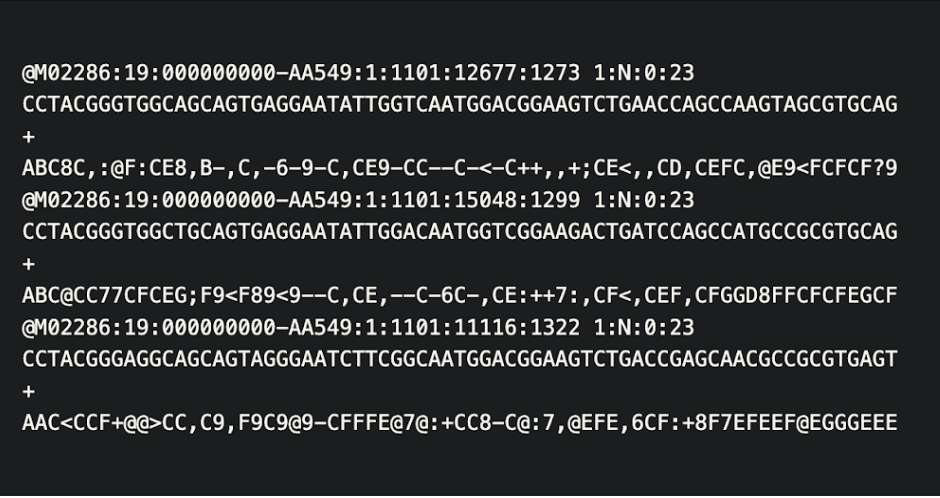
\includegraphics[width=0.7\textwidth,height=\textheight]{images/fastqfile.png}
\caption{A part of a D. melanogaster FASTQ file.}
\end{figure}

\hypertarget{the-fastqc-software}{%
\subsection{The FASTQC software}\label{the-fastqc-software}}

\begin{itemize}
\tightlist
\item
  \href{https://www.bioinformatics.babraham.ac.uk/projects/fastqc/}{FastQC}
  aims to provide a QC report which can spot problems which originate
  either in the sequencer or in the starting library material.
\end{itemize}

\begin{figure}
\centering
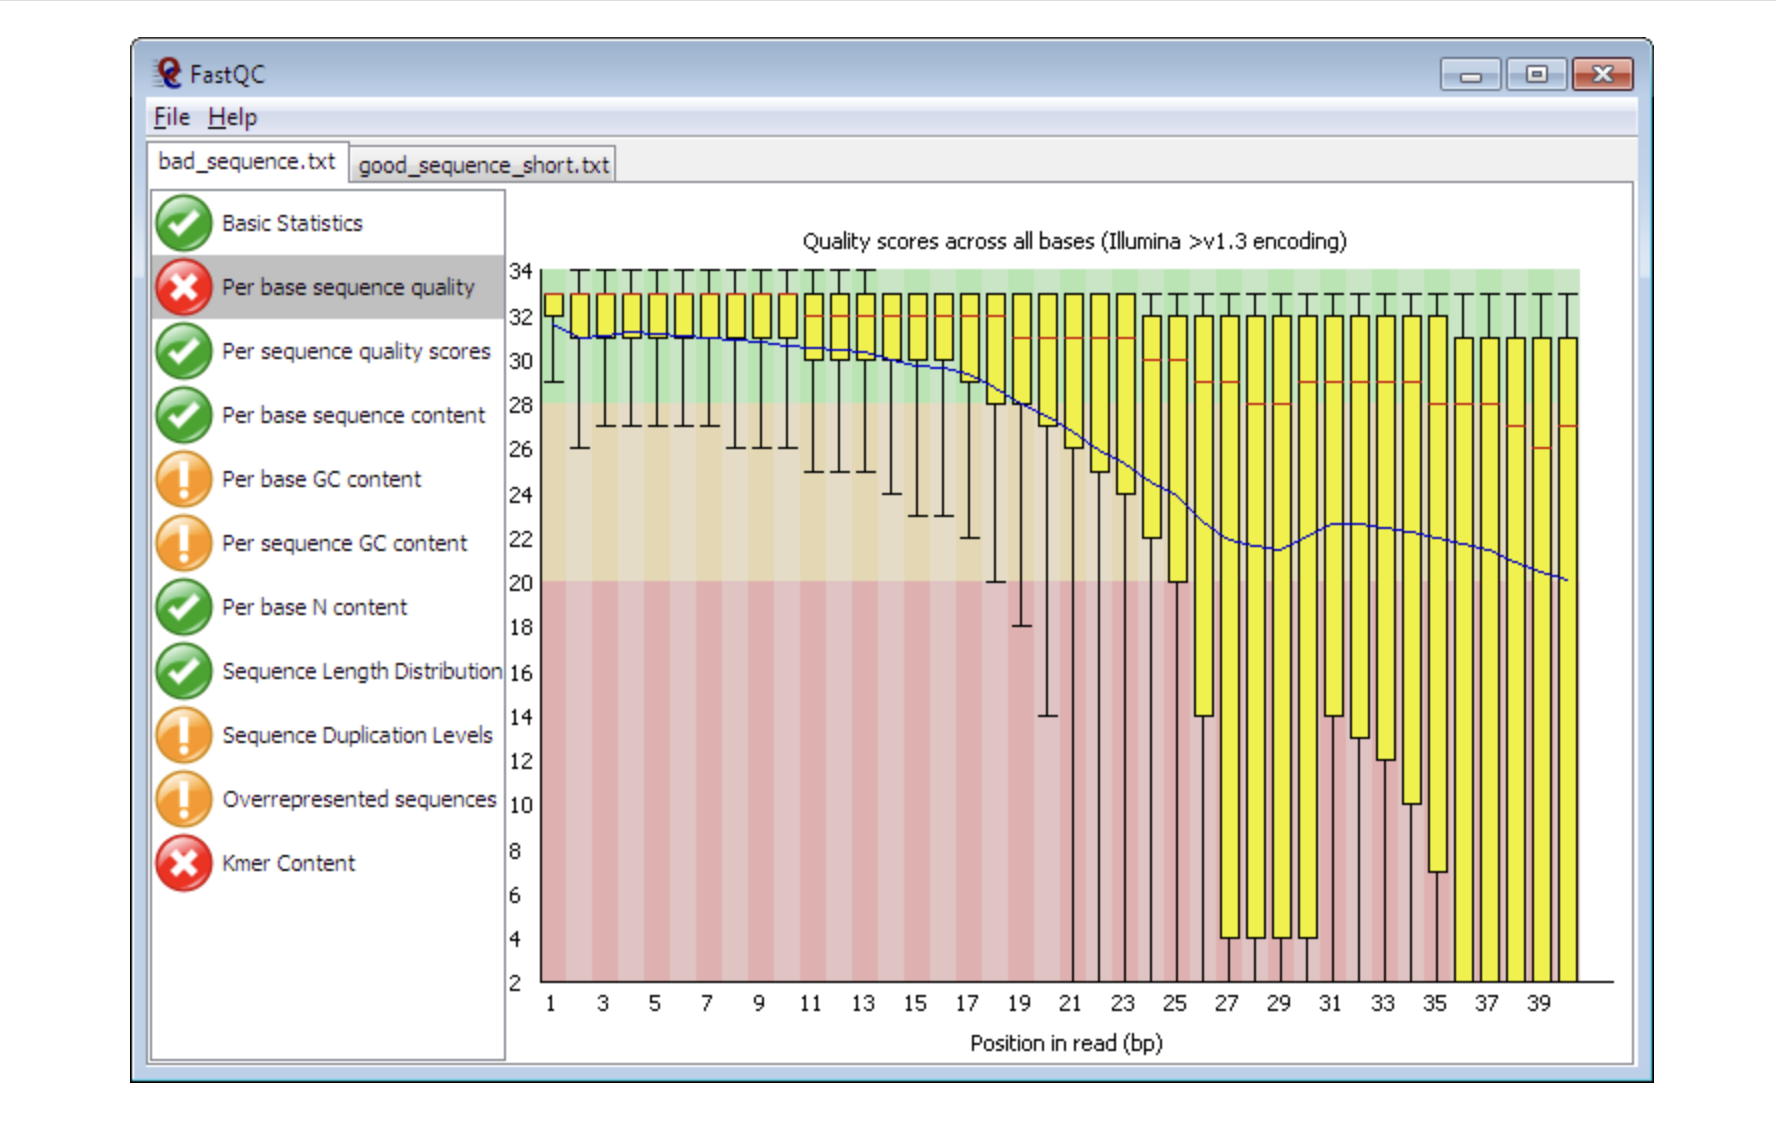
\includegraphics[width=0.7\textwidth,height=\textheight]{images/fastqc.png}
\caption{Interactive version of fastqc. Not scalable to large datasets.}
\end{figure}

\begin{itemize}
\item
  FastQC can be run in one of two modes: as a stand-alone interactive
  application for the immediate analysis of small numbers of FastQ
  files, or in a non-interactive mode (aka \textbf{command line}!) where
  it would be suitable for integrating into a \textbf{larger analysis
  pipeline} for the systematic processing of large numbers of files.
\item
  Most of the information in this section was taken directly from the
  FASTQC manual.
\end{itemize}

The main functions of FastQC are:

\begin{itemize}
\tightlist
\item
  Import of data from BAM, SAM or FastQ files (any variant)
\item
  Providing a quick overview to tell you in which areas there may be
  problems
\item
  Summary graphs and tables to quickly assess your data
\item
  Export of results to an HTML based permanent report
\item
  The Basic Statistics module generates some simple composition
  statistics for the file analyzed:
\item
  Filename: The original filename of the file which was analyzed\\
\item
  File type: Says whether the file appeared to contain actual base calls
  or colorspace data which had to be converted to base calls\\
\item
  Encoding: Says which ASCII encoding of quality values was found in
  this file.\\
\item
  Total Sequences: A count of the total number of sequences processed.
  There are two values reported, actual and estimated.
\item
  Filtered Sequences: If running in Casava mode sequences flagged to be
  filtered will be removed from all analyses. The number of such
  sequences removed will be reported here. The total sequences count
  above will not include these filtered sequences.
\item
  Sequence Length: Provides the length of the shortest and longest
  sequence in the set. If all sequences are the same length only one
  value is reported.
\item
  \%GC: The overall \%GC of all bases in all sequences
\item
  Tiles: Illumina flowcells are divided into tiles. To see if there is a
  loss in quality associated with specific parts of the flowcell, FASTQC
  calculates average quality scores for each tile across all positions
  in the reads.
\end{itemize}

\hypertarget{what-about-fastqe}{%
\subsubsection{What about FASTQE?}\label{what-about-fastqe}}

\begin{itemize}
\item
  \href{https://fastqe.com/}{FASTQE} is a program that analyzes FASTQ
  files \& reads out an emoji output as an indicator of the sequence's
  quality in the file. So, a high quality read may look like a smily
  face, while the poop symbol indicates\ldots{} well you get the idea.
\item
  Like the popular FastQC software, FASTQE can be used to analyze FASTQ
  file quality whether it's from a genome sequencing project, an RNA-seq
  project, a ChIP-seq project, etc.
\item
  The FASTQE program is limited to short read NGS data of 500bp/read or
  less.
\end{itemize}

\hypertarget{the-data-we-are-looking-at}{%
\subsection{The Data we are looking
at}\label{the-data-we-are-looking-at}}

\begin{itemize}
\item
  Here's a brief background on the in-class metagenomics project that
  Dr.~Enke's Bio 481 Genomics class at James Madison University is
  collecting data for. Garter snakes excrete sexually dimorphic
  pheromones to attract a mate.
\item
  The hypothesis of their experiment is that male and female garter
  snakes host unique microbial communities in their musk glands that
  contribute to sexually dimorphic bioengineering of these pheromone
  molecules.
\end{itemize}

\begin{center}\rule{0.5\linewidth}{0.5pt}\end{center}

\hypertarget{lets-install-fastqe}{%
\subsection{Let's install fastqe}\label{lets-install-fastqe}}

\hypertarget{step-1-install-the-fastqe-software}{%
\subsection{Step 1: Install the fastqe
software}\label{step-1-install-the-fastqe-software}}

In your terminal, type:

\begin{Shaded}
\begin{Highlighting}[]
\ExtensionTok{pip}\NormalTok{ install fastqe}
\end{Highlighting}
\end{Shaded}

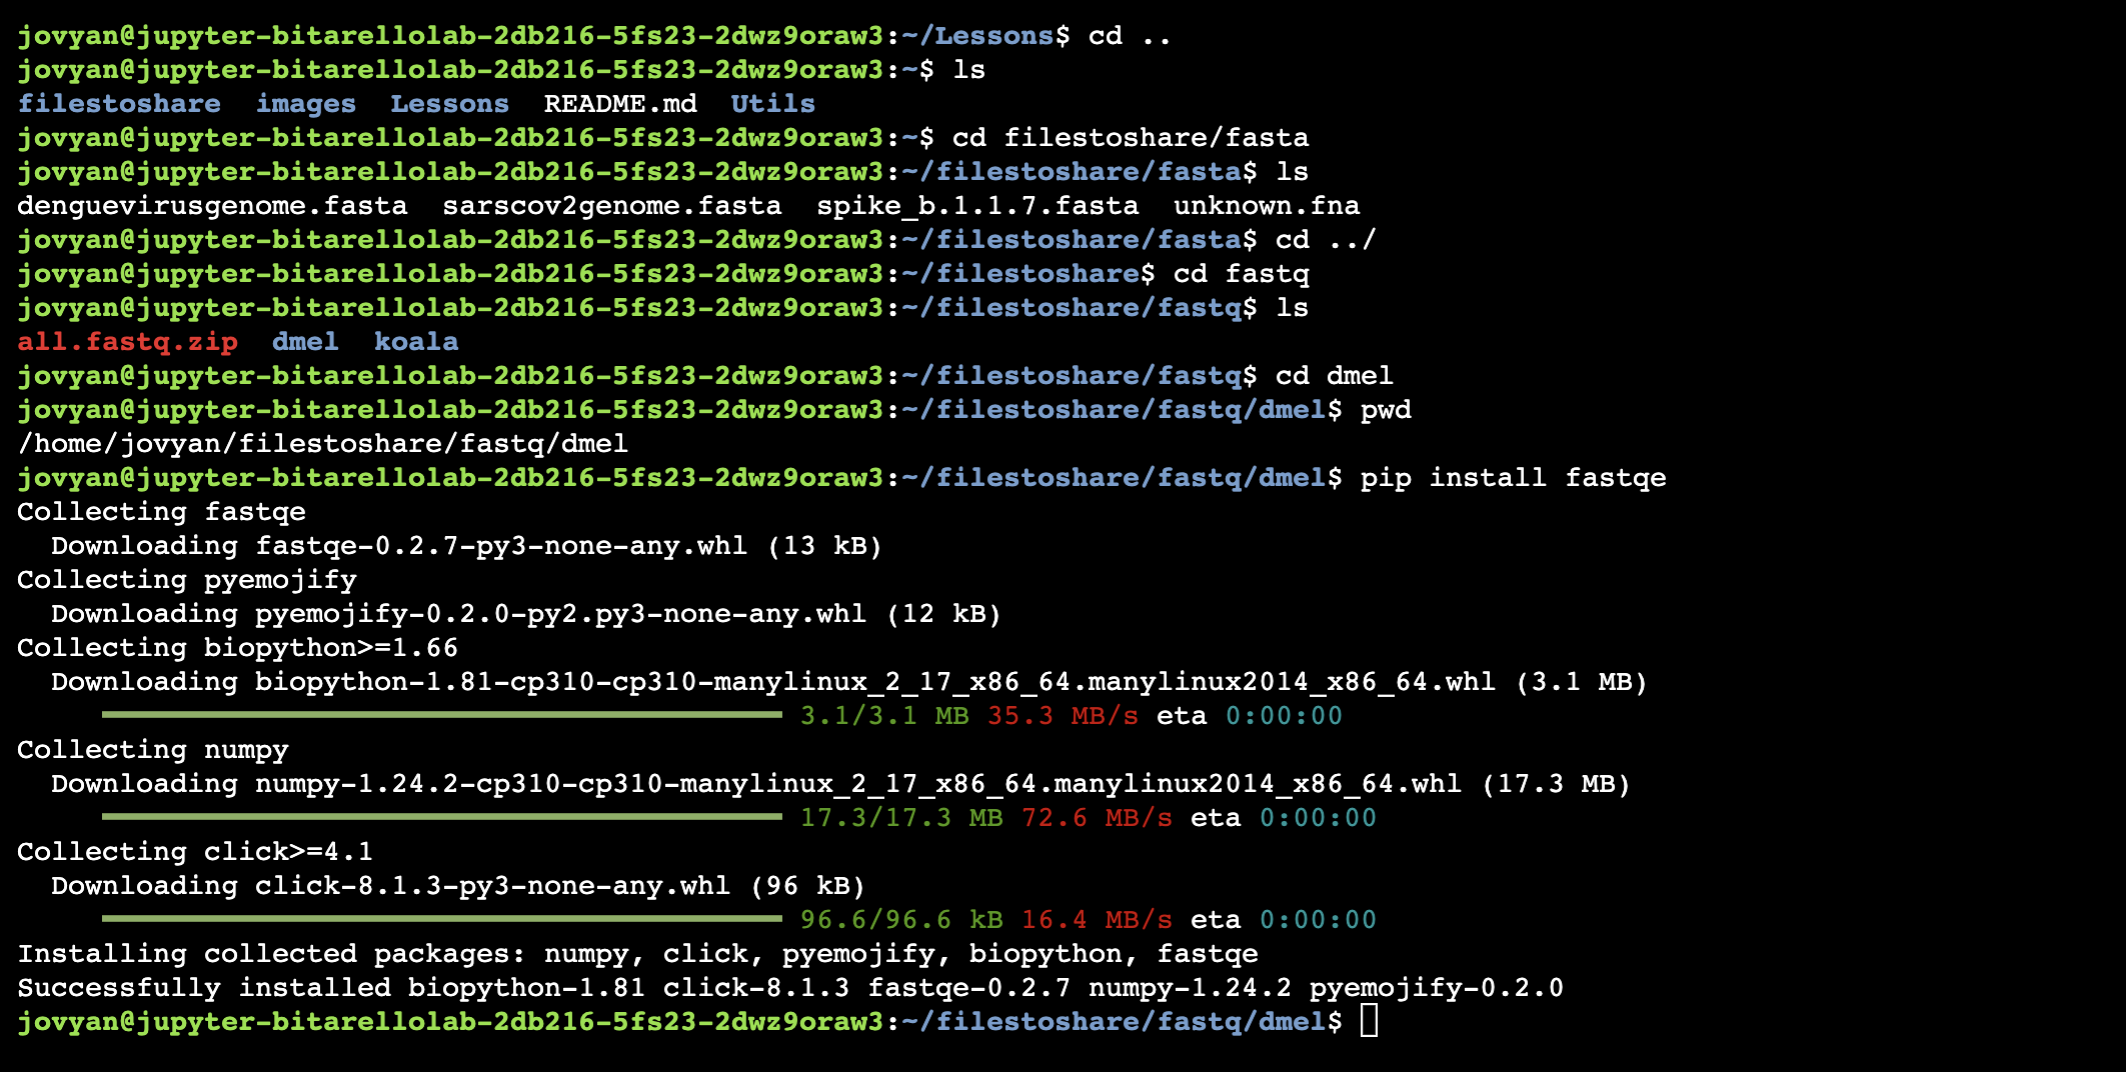
\includegraphics{images/install_fastqe.png}

\hypertarget{step-2-running-fastqe}{%
\subsection{Step 2: Running fastqe}\label{step-2-running-fastqe}}

\begin{itemize}
\item
  Task: Run the fastqe program to generate your emoji fastq report.
\item
  Usage: fastqe {[}fastq-file{]} (run the fastqe program. If a wildcard
  {[}e.g.~*.fastq{]} is provided, fastqe will run on all the fastq files
  in the current working directory.
\end{itemize}

Note: Remember that fastq files are very large, so this command will
take \textasciitilde30 seconds/

First, list what's in this directory:

\begin{Shaded}
\begin{Highlighting}[]
\ExtensionTok{fastqe} \PreprocessorTok{*}\NormalTok{fastq}
\end{Highlighting}
\end{Shaded}

**Q12) What are the advantages and disadvantages to using the command
fastqe *.fastq rather than fastqe for each of your files (e.g.~fastqe
Female2-oral1.fastq \ldots{} fastqe Male5-oral1.fastq\ldots) ?**

\textbf{Q13) Which one of the three files seems to have lower quality
than the others?}

\hypertarget{step-3-using-the-help-page}{%
\subsection{Step 3: Using the help
page}\label{step-3-using-the-help-page}}

Open the FASTQE help page to view the ``optional arguments'', these are
all of the options and setting for the program.

To get the help info for fastqe (and many other command line programs)
add the --help option to the fastqe program instead of a filename or
wildcard (remember to leave a space between fastqe and --help).

\begin{Shaded}
\begin{Highlighting}[]
\CommentTok{\#type your command in your terminal}
\end{Highlighting}
\end{Shaded}

You should see something like this:

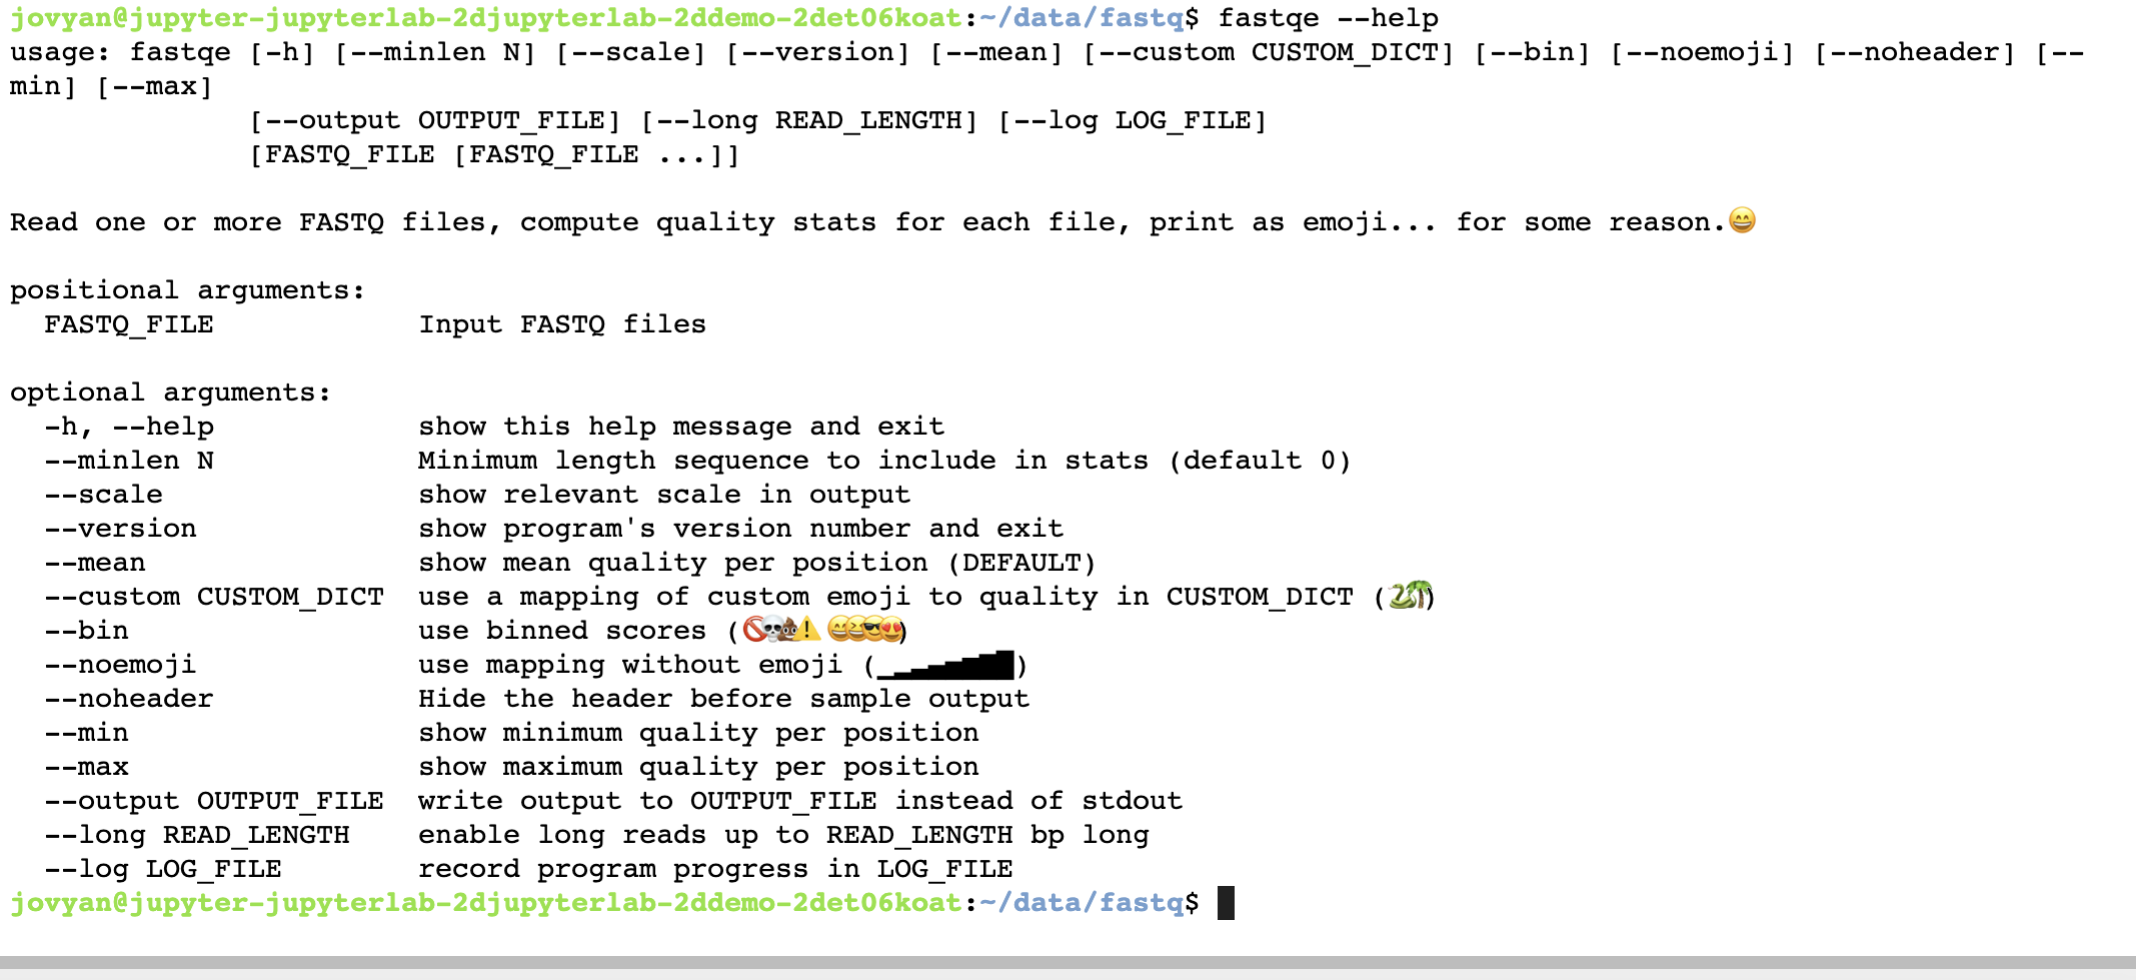
\includegraphics{images/fastqe_help.png}

Which optional argument will show the version \# of FASTQE?

\hypertarget{step-4.-scale}{%
\subsection{Step 4. Scale}\label{step-4.-scale}}

Add the --scale option to the fastqe command to view the Phred score
associated with each emoji in your output. Try this just for the
\texttt{Male5-oral1.fastq} file (remember to leave a space before you
type --scale). This will take a few seconds to run.

\begin{Shaded}
\begin{Highlighting}[]
\CommentTok{\#type your command in your terminal}
\ExtensionTok{fastqe}\NormalTok{ Male5{-}oral1.fastq }\AttributeTok{{-}{-}scale}
\end{Highlighting}
\end{Shaded}

\hypertarget{step-5.-quality}{%
\subsubsection{Step 5. Quality}\label{step-5.-quality}}

The quality, also called phred score, is the probability that the
corresponding basecall is incorrect.

Phred scores use a logarithmic scale, and are represented by ASCII
characters, mapping to a quality usually going from 0 to 40.

\begin{figure}
\centering
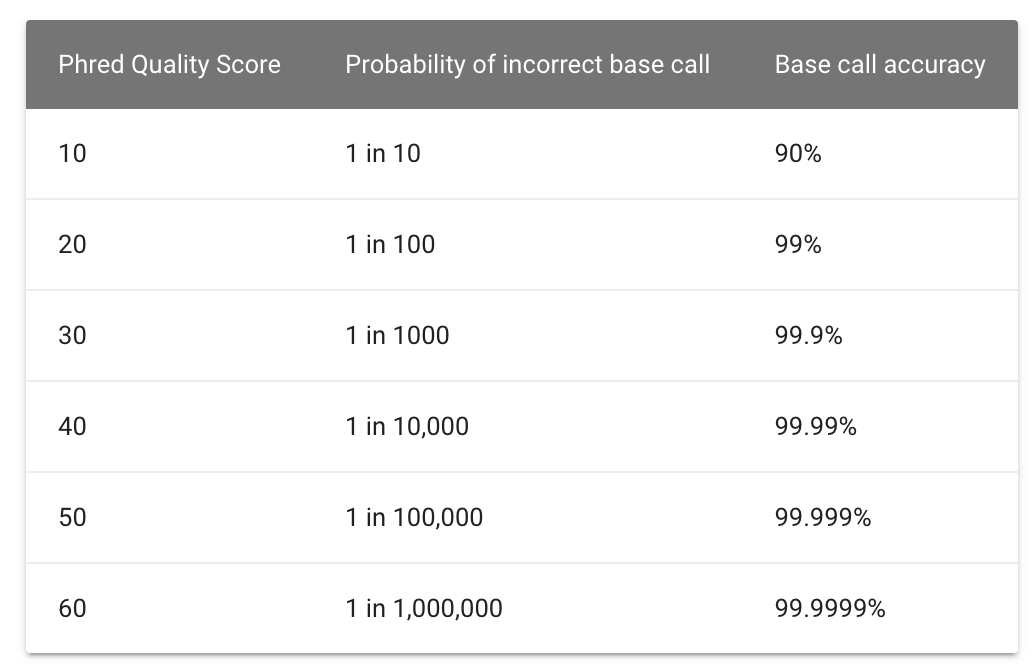
\includegraphics{images/phred.png}
\caption{Credit:\url{https://www.hadriengourle.com/tutorials/file_formats/\#the-fastq-format}}
\end{figure}

\textbf{Q13) Phred score of ≤20 is considered a poor quality base call.
How many poor quality base calls are at the 3' end of this read?}

\hypertarget{step-6.-fastp}{%
\subsection{Step 6. FASTP}\label{step-6.-fastp}}

Now let's try a different tool, called fastp. But first, we need to
install some pre-req libraries.

Paste into your command line

\begin{Shaded}
\begin{Highlighting}[]
\ExtensionTok{conda}\NormalTok{ config }\AttributeTok{{-}{-}add}\NormalTok{ channels bioconda}
\ExtensionTok{conda}\NormalTok{ config }\AttributeTok{{-}{-}add}\NormalTok{ channels conda{-}forge}
\ExtensionTok{pip}\NormalTok{ install nodejs}
\ExtensionTok{pip}\NormalTok{ install scikit{-}learn}
\ExtensionTok{pip}\NormalTok{ install tensorflow}
\ExtensionTok{conda}\NormalTok{ create }\AttributeTok{{-}n}\NormalTok{ assembly }\AttributeTok{{-}c}\NormalTok{ conda{-}forge }\AttributeTok{{-}c}\NormalTok{ bioconda fastp }\AttributeTok{{-}y}
\ExtensionTok{conda}\NormalTok{ activate assembly}
\end{Highlighting}
\end{Shaded}

FASTP gives a more conventional readout of the .fastq file data. Fastp
is similar to the famous FastQC; however, it also has a trimming tool to
cut out or filtering the low quality sequences in our file.

Run fastp on the lower quality \texttt{Male5-oral1.fastq} file.

\begin{verbatim}
 Usage (Note: You will need to use all of these elements in your command):

fastp is the name of software that will check the quality of the fastq file
 -i [input.fastq] -i option specifies the input file for fastp
 -o [ouput.fastq] -o option specifies the ouput file for fastp
 --html [ouput.html] --html option specifies the name of the HTML report for fastp
 --json [ouput.json] --json option specifies the name of the JSON report for fastp
\end{verbatim}

Write a command using Male5-oral1.fastq as your input and
out.Male5-oral1.fastq as your output. Name your --html report
Male5-oral1.html and your --json report Male5-oral1.json.

\begin{Shaded}
\begin{Highlighting}[]
\NormalTok{\#type your command into your command line}
\end{Highlighting}
\end{Shaded}

You should now have 3 new files in your fastp folder

\begin{itemize}
\tightlist
\item
  .html file (this is your QC report)
\item
  .json file (ignore this for now)
\item
  trimmed fastq file (out.Male5\_oral1.fastq)
\end{itemize}

Click on the fastp.html file in the left sidebar pane inside
\texttt{filestoshare/fastq/} on the left to examine this report.

\textbf{Q14) From the ``Summary'' data in your HTML fastp report, how
many reads are in this FASTQ file before and after filtering?}

\begin{center}\rule{0.5\linewidth}{0.5pt}\end{center}

\hypertarget{learn-more}{%
\section{Learn More}\label{learn-more}}

FASTQE Official Webpage. \url{https://fastqe.com/}

FASTP Github Repository. \url{https://github.com/OpenGene/fastp}

FASTQ files and Quality Control.
\url{https://datacarpentry.org/wrangling-genomics/02-quality-control/index.html}

\end{document}
